% EcoVoz paper. Numbers, tables and figures come from scripts/make_report.py.
% Build:  tectonic main.tex   (or upload the folder to Overleaf together with ../reports/figures)
\documentclass[conference]{IEEEtran}
\usepackage{iftex}
\ifPDFTeX
  \usepackage[utf8]{inputenc}
  \usepackage[T1]{fontenc}
\else
  \usepackage{fontspec}
  \setmainfont{texgyretermes}[Extension=.otf, UprightFont=*-regular, BoldFont=*-bold,
    ItalicFont=*-italic, BoldItalicFont=*-bolditalic]
\fi
\usepackage[english]{babel}
\usepackage{amsmath,amssymb}
\usepackage{booktabs}
\usepackage{array}
\usepackage{graphicx}
\usepackage{cite}
\usepackage{xurl}
\usepackage{tikz}
\usetikzlibrary{arrows.meta,positioning}
\usepackage[hidelinks]{hyperref}

\graphicspath{{../reports/figures/}{figures/}}
\newcommand{\ImgTotal}{6108}
\newcommand{\ImgGroups}{5611}
\newcommand{\ImgInGroups}{765}
\newcommand{\AudioTotal}{20514}
\newcommand{\AudioTrain}{18779}
\newcommand{\AudioHours}{22.5}
\newcommand{\AudioLeak}{2077}
\newcommand{\ResAcc}{91.0}
\newcommand{\ResF}{90.6}
\newcommand{\MobAcc}{92.4}
\newcommand{\MobF}{92.5}
\newcommand{\DefaultModel}{MobileNetV3-L}
\newcommand{\BestTemp}{0.74}
\newcommand{\EceBefore}{5.0}
\newcommand{\EceAfter}{1.5}
\newcommand{\RejectCoverage}{91.5}
\newcommand{\RejectAcc}{96.7}
\newcommand{\McP}{= 0.111}
\newcommand{\McA}{22}
\newcommand{\McB}{35}
\newcommand{\ValSlrWer}{20.5}
\newcommand{\ValSlrCer}{6.0}
\newcommand{\SlrWer}{24.6}
\newcommand{\SlrCer}{7.9}
\newcommand{\SlrWerGreedy}{35.1}
\newcommand{\SlrWerLow}{22.4}
\newcommand{\SlrWerHigh}{26.8}
\newcommand{\TuxWer}{8.7}
\newcommand{\TuxCer}{1.8}
\newcommand{\Alpha}{0.8}
\newcommand{\Beta}{1.0}
\newcommand{\SpeechParams}{23.2}
\newcommand{\SpeechBestEpoch}{50}
\newcommand{\VideoFps}{106.3}
\newcommand{\VideoFpsCpu}{84.2}
\newcommand{\VideoAcc}{77.7}
\newcommand{\OwnBottleMob}{100.0}
\newcommand{\OwnBottleFrames}{184}
\newcommand{\OwnBottleRes}{5.4}
\newcommand{\OwnNotebookMob}{67.7}
\newcommand{\OwnNotebookFrames}{217}
\newcommand{\OwnNotebookRes}{0.5}
\newcommand{\AudioLat}{0.07}
\newcommand{\AudioLatCpu}{0.30}
\newcommand{\HwCpu}{AMD Ryzen 5 7600 6-Core Processor}
\newcommand{\HwGpu}{NVIDIA GeForce RTX 5060}
\newcommand{\ExpScratchWer}{101.5}
\newcommand{\ExpScratchCer}{45.0}
\newcommand{\ExpAugWer}{97.1}
\newcommand{\ExpAugCer}{46.7}
\newcommand{\ExpTuxWer}{81.2}
\newcommand{\ExpTuxCer}{32.4}
\newcommand{\ExpTransferWer}{62.8}
\newcommand{\ExpTransferCer}{19.7}
\newcommand{\ExpMultiWer}{29.9}
\newcommand{\ExpMultiCer}{7.8}


% Student IDs (carnés): defined in carnes.tex, which is not published in the repository.
\newcommand{\carneA}{}
\newcommand{\carneB}{}
\newcommand{\carneC}{}
\IfFileExists{carnes.tex}{\input{carnes}}{}

\begin{document}

\title{EcoVoz: Visual Waste Classification and CTC-Based Spanish Speech Recognition in a Multimodal Application}

\author{
\IEEEauthorblockN{Anthony Jafeth Arias Robleto\carneA, Randy Espinoza Downing\carneB,\\ Kenneth Jhoan Araya Arguedas\carneC}
\IEEEauthorblockA{School of Computer Engineering, Instituto Tecnológico de Costa Rica\\
San Carlos Local Technological Campus\\
IC-6200 Artificial Intelligence, Second Semester 2026. Prof. Ing. Efrén Jiménez Delgado}}

\maketitle

\begin{abstract}
Se presenta EcoVoz, una aplicación local que clasifica residuos en imágenes y video y transcribe voz en español. Para visión se compararon ResNet-50 y MobileNetV3-Large con cuatro estrategias de transfer learning sobre \ImgTotal{} imágenes de seis clases, particionadas por grupos de fotos casi idénticas. En prueba alcanzaron \ResAcc\,\% y \MobAcc\,\% de accuracy, una diferencia que no es estadísticamente significativa, y la red móvil es unas cinco veces más liviana. Para voz se entrenó un DeepSpeech2 con pérdida CTC. Con solo 100 audios el CER de validación en locutores nuevos fue de \ExpScratchCer\,\% y bajó a \ExpTransferCer\,\% al partir de un modelo preentrenado. El modelo final, con \AudioTrain{} audios de entrenamiento, obtuvo en prueba un WER de \SlrWer\,\% y un CER de \SlrCer\,\% con locutores y frases no vistos, y \TuxWer\,\% y \TuxCer\,\% con frases nuevas de un locutor conocido. En el equipo de la demostración el video se procesa a \VideoFps{} cuadros por segundo con GPU y \VideoFpsCpu{} sin ella, y un audio se transcribe en menos de medio segundo (percentil 95), por encima de los requisitos de tiempo casi real.
\end{abstract}

\begin{IEEEkeywords}
transfer learning, clasificación de residuos, reconocimiento automático del habla, CTC, DeepSpeech2, aplicación multimodal
\end{IEEEkeywords}

\section{Introduction}

Sorting waste at the source requires a small decision that is repeated many times: which bin each object goes into. An assistant that sees the object and listens to the person can support that decision, but it needs models from two different domains. Computer vision has pretrained feature extractors that can be adapted with few images. Speech recognition must, in addition, solve the alignment between a long signal and a short text whose temporal correspondence is unknown.

This work presents \emph{EcoVoz}, a local application that integrates three modalities: images, video classified frame by frame, and audio transcribed to text. We address three questions:
\begin{enumerate}
\item how much does each level of fine-tuning contribute in transfer learning, and is a large network (ResNet-50) justified over a mobile one (MobileNetV3-Large)?
\item what can a CTC model learn from only 100 recordings, and how much do data augmentation and pretraining help?
\item is a desktop computer enough to respond in near real time across the three modalities?
\end{enumerate}

The contributions are a comparison of eight vision configurations on a single object-grouped split, a series of five speech experiments evaluated on the same unseen speakers, an end-to-end latency measurement on GPU and CPU, and a repository with the code that produces every figure in this paper.

The rest of the paper is organized as follows: Section~\ref{sec:teoria} summarizes the theoretical background, Section~\ref{sec:metodo} describes the data, models, training, and application, Section~\ref{sec:resultados} analyzes the results, and Section~\ref{sec:conclusiones} concludes.

\section{Background}\label{sec:teoria}

\subsection{Transfer Learning}
The first layers of a convolutional network learn edges and textures that are useful for almost any visual task, while the last layers specialize in the source classes~\cite{yosinski}. It is therefore possible to reuse a network trained on ImageNet~\cite{imagenet}, replace its head, and train only part of it. Freezing more layers reduces overfitting when data are scarce, and unfreezing them allows the features to adapt to the new domain.

ResNet-50~\cite{resnet} learns residuals $\mathcal{F}(x)$ and outputs $\mathcal{F}(x)+x$, which makes it possible to train deep networks without gradient degradation. MobileNetV3~\cite{mobilenet} uses depthwise separable convolutions, inverted residual blocks, and channel attention to reduce operations and parameters.

\subsection{Connectionist Temporal Classification}
Let $y^t_k$ be the probability of symbol $k$ at step $t$, over an alphabet extended with the blank $\epsilon$. A path $\pi$ assigns one symbol to each step, and the function $\mathcal{B}$ reduces it to text by merging repetitions and removing blanks. CTC~\cite{ctc} defines the probability of a transcription $\ell$ as the sum over all of its paths:
\begin{equation}
p(\ell\mid x)=\sum_{\pi:\,\mathcal{B}(\pi)=\ell}\ \prod_{t=1}^{T} y^t_{\pi_t}.
\end{equation}
The sum is computed by dynamic programming in $O(T|\ell|)$, and the loss is $-\ln p(\ell\mid x)$. Training thus requires no labels for when each letter is spoken. The blank makes it possible to represent double letters: producing ``ll'' requires at least one $\epsilon$ between them.

\subsection{Decoding}
Greedy decoding takes the most probable symbol at each step. It is fast, but it ignores that several paths add up to the same text. Prefix beam search~\cite{beam} sums those paths and admits a language model, with the criterion
\begin{equation}
\hat{\ell}=\arg\max_{\ell}\ \ln p(\ell\mid x)+\alpha\ln p_{LM}(\ell)+\beta|\ell|,
\end{equation}
where $\alpha$ weights the language model and $\beta$ offsets its preference for short texts.

\subsection{DeepSpeech2}
DeepSpeech2~\cite{ds2} maps a spectrogram to character probabilities using 2D convolutions, which capture local time--frequency patterns and reduce resolution, followed by bidirectional recurrent layers, which provide context in both directions. It is the architecture studied in the course~\cite{keras-ctc}.

\subsection{Metrics}
Classification uses accuracy, precision, recall, and F1. Macro F1 averages the classes without weighting, so a minority class counts as much as the others. Speech uses the edit distance between reference and hypothesis:
\begin{equation}
\mathrm{WER}=\frac{S+D+I}{N},
\end{equation}
where $S$, $D$, and $I$ are word substitutions, deletions, and insertions, and $N$ is the number of reference words. CER is the equivalent over characters. WER penalizes an entire word for a single wrong letter, so it is usually considerably higher.

\section{Methodology}\label{sec:metodo}

\subsection{Image Dataset}
We merged TrashNet~\cite{trashnet} (MIT license, white background) and the six equivalent classes of RealWaste~\cite{realwaste} (CC BY-NC-SA 4.0, real waste from a materials recovery facility): \ImgTotal{} images labeled by their authors (Fig.~\ref{fig:examples}). Mixing both sources avoids depending on a single background.

Exact duplicates were removed by pixel hash. Since both datasets contain several photos of the same object, a random split would leak information. We computed embeddings with a pretrained ResNet-50 and merged into connected components the same-source pairs with a cosine similarity of 0.88 or higher, a threshold chosen by inspecting real pairs. This yielded \ImgGroups{} groups, with \ImgInGroups{} images in groups of two or more. Each group was assigned as a whole to a 70/15/15 split, stratified by class and source (Table~\ref{tab:images}).

\begin{figure*}[t]
\centering
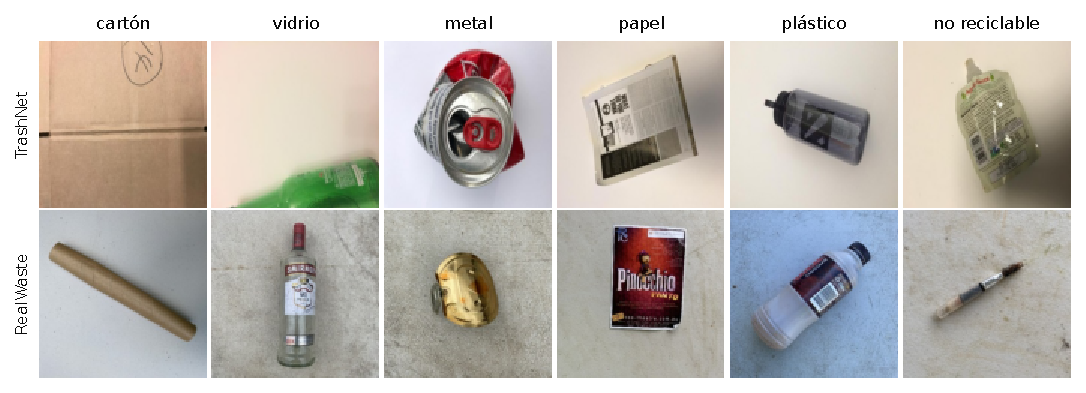
\includegraphics[width=0.76\textwidth]{dataset_examples.pdf}
\caption{Training examples by class and source. The background and the condition of the objects differ between the two datasets.}
\label{fig:examples}
\end{figure*}

\begin{table}[t]
\centering
\caption{Images per class and split}
\label{tab:images}
\begin{tabular}{lrrrr}
\toprule
Class & Train & Val. & Test & Total \\
\midrule
cardboard & 604 & 130 & 130 & 864 \\
glass & 642 & 138 & 138 & 918 \\
metal & 837 & 181 & 181 & 1199 \\
paper & 766 & 164 & 164 & 1094 \\
plastic & 980 & 211 & 210 & 1401 \\
non-recyclable & 441 & 96 & 95 & 632 \\
\textbf{Total} & 4270 & 920 & 918 & 6108 \\
\bottomrule
\end{tabular}

\end{table}

\subsection{Speech Dataset}
Two sources were combined. The first is a random sample of 12\,000 recordings from TUX~\cite{tux}, the course's class dataset, with a single speaker. The second is the Latin American OpenSLR 72, 73, and 74 corpora~\cite{openslr} (Colombia, Peru, and Puerto Rico, CC BY-SA 4.0). Everything was converted to 16\,kHz, 16-bit mono WAV, leading and trailing silence was trimmed, and clips of 0.7 to 12\,s were kept. Transcriptions were normalized to lowercase, without punctuation, over a 34-symbol alphabet that keeps accents, \emph{ü}, and \emph{ñ}. The result is \AudioTotal{} recordings and \AudioHours{} hours (Table~\ref{tab:audio}).

In OpenSLR, the same sentence is read by up to 94 people. One speaker per country and sex was held out for validation and another for testing, and every held-out sentence was removed from training, regardless of who read it. This control, together with the remaining recordings of the held-out speakers, discarded \AudioLeak{} recordings. In TUX the split is by sentence, so its metrics are reported separately: they measure new sentences, but not new speakers.

\begin{table}[t]
\centering
\caption{Recordings per split}
\label{tab:audio}
\begin{tabular}{lrrrr}
\toprule
Partición & OpenSLR & TUX & Locut. & Horas \\
\midrule
Entrenamiento & 8347 & 10432 & 67 & 20,6 \\
Validación & 300 & 583 & 6 & 1,0 \\
Prueba & 278 & 574 & 6 & 0,9 \\
\bottomrule
\end{tabular}

\end{table}

\subsection{Vision Models and Fine-Tuning}
ResNet-50 and MobileNetV3-Large were compared with ImageNet weights, the same split, seed, preprocessing (short side of 256 and a 224-pixel crop), and epoch budget. In both, the head was replaced by a six-output layer with a dropout of 0.3. To justify the fine-tuning strategy, four were tested:
\begin{itemize}
\item \emph{head only}: frozen extractor;
\item \emph{last blocks, no augmentation}: \texttt{layer3} and \texttt{layer4} are unfrozen in ResNet, or blocks 11 to 16 in MobileNet;
\item \emph{last blocks, with augmentation};
\item \emph{full network, with augmentation}.
\end{itemize}
The last three first train the head for four epochs at a rate of $10^{-3}$, so that random gradients do not destroy the pretrained weights. They then fine-tune the extractor at a lower rate ($1.5\times10^{-4}$ if partial, $10^{-4}$ if full) than the head ($5\times10^{-4}$). Frozen layers keep their BatchNorm statistics fixed.

We used AdamW, cosine decay, up to 30 epochs with early stopping (patience 8), label smoothing of 0.05, and class weights proportional to the square root of the inverse frequency. Augmentation simulates a camera: random cropping, flips, rotation, perspective, lighting, blur, and random erasing. The strategy was chosen by validation macro F1. Confidence was calibrated on validation with \emph{temperature scaling}~\cite{calibration}.

\subsection{Speech Model}
The input is an 80-band log-mel spectrogram (25\,ms window, 10\,ms hop, Fig.~\ref{fig:spectrogram}), with pre-emphasis and per-utterance normalization that ignores batch padding. The network follows the DeepSpeech2 seen in class: two convolutions of $11\times41$ and $11\times21$ (time by frequency) with 32 filters and strides $(2,2)$ and $(1,2)$, five bidirectional GRUs of 512 units, a dense layer, and a log-softmax output, for a total of \SpeechParams{} million parameters. The output has 50 steps per second. It is implemented in PyTorch rather than Keras because TensorFlow offers no GPU support on native Windows.

\begin{figure}[t]
\centering
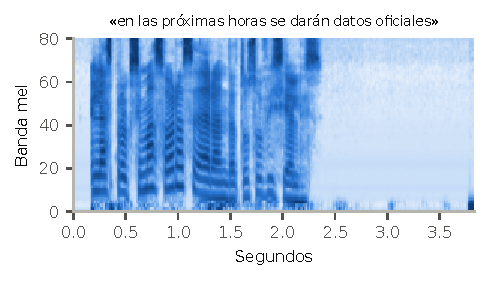
\includegraphics[width=\columnwidth]{spectrogram.pdf}
\caption{Normalized log-mel spectrogram of a test recording.}
\label{fig:spectrogram}
\end{figure}

Five experiments were trained, all selected by validation CER:
\begin{enumerate}
\item 100 Latin American recordings from scratch, with a reduced network (three GRUs of 256);
\item the same 100 recordings with augmentation;
\item pretraining on TUX only;
\item the same 100 recordings starting from the pretrained model;
\item final model: the \AudioTrain{} recordings, starting from the pretrained model.
\end{enumerate}
Augmentation combines speed perturbation ($\pm$12\,\%), noise with an SNR of 10 to 35\,dB, and SpecAugment~\cite{specaugment}. We used AdamW with warm-up, plateau, and cosine decay, gradient clipping at 5, and mixed precision, computing CTC in 32 bits.

The language model is an interpolated character 6-gram, estimated only from training texts. The values $\alpha$ = \Alpha{} and $\beta$ = \Beta{} were chosen on validation.

\subsection{Application}
Fig.~\ref{fig:architecture} summarizes the application, built with Gradio~\cite{gradio}. It has tabs for images (file, camera, or clipboard), frame-by-frame video, live camera, audio (microphone or file), and results. In video, every frame is classified and only the displayed label is smoothed with an exponential moving average. If the calibrated confidence does not reach the threshold, the application replies that it is not sure. Recordings longer than 10\,s are split at the quietest pause near the limit. Models are stored in 16 bits and nothing is sent to the Internet.

\begin{figure}[t]
\centering
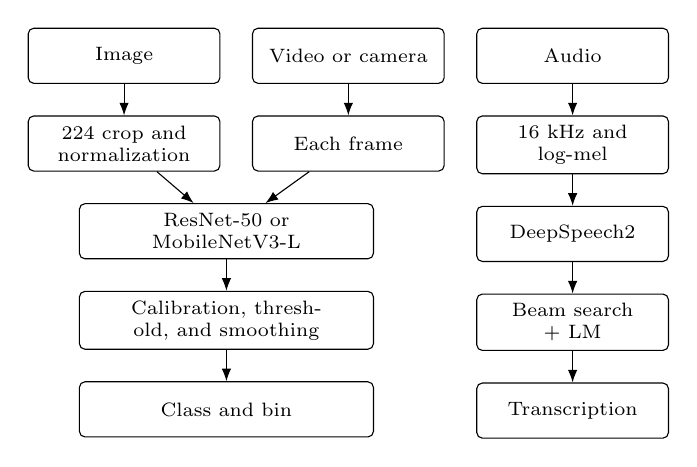
\begin{tikzpicture}[
  box/.style={draw, rounded corners=2pt, align=center, font=\scriptsize, minimum height=7mm, text width=22mm},
  flow/.style={-{Latex[length=1.6mm]}}, node distance=4mm]
\node[box] (image) {Image};
\node[box, right=of image] (video) {Video or camera};
\node[box, right=of video] (audio) {Audio};
\node[box, below=of image] (crop) {224 crop and normalization};
\node[box, below=of video] (frames) {Each frame};
\node[box, below=of audio] (mel) {16 kHz and log-mel};
\node[box, below=of crop, xshift=13mm, text width=35mm] (cnn) {ResNet-50 or MobileNetV3-L};
\node[box, below=of mel] (ds) {DeepSpeech2};
\node[box, below=of cnn, text width=35mm] (cal) {Calibration, threshold, and smoothing};
\node[box, below=of ds] (beam) {Beam search + LM};
\node[box, below=of cal, text width=35mm] (class) {Class and bin};
\node[box, below=of beam] (text) {Transcription};
\draw[flow] (image) -- (crop);
\draw[flow] (video) -- (frames);
\draw[flow] (audio) -- (mel);
\draw[flow] (crop) -- (cnn);
\draw[flow] (frames) -- (cnn);
\draw[flow] (mel) -- (ds);
\draw[flow] (cnn) -- (cal);
\draw[flow] (ds) -- (beam);
\draw[flow] (cal) -- (class);
\draw[flow] (beam) -- (text);
\end{tikzpicture}
\caption{Flow of the three modalities within the application.}
\label{fig:architecture}
\end{figure}

\subsection{Origin of the Models}
No model is used as downloaded from the Internet. In vision, the only external component is torchvision's ImageNet weights, the starting point that transfer learning requires, as in the class 11 notebook. The six-class output layer is new, randomly initialized, and was trained on our data together with the unfrozen blocks (Section~\ref{sec:metodo}-C). In ResNet-50, the rest of the extractor was unchanged. In speech, no external pretrained model was used: DeepSpeech2 starts from random weights, and all of its parameters, including the TUX pretraining, were trained in this work with the CTC loss. The language model and the calibration temperature were also computed here, from the training and validation sets.

\subsection{Evaluation Protocol and Reproducibility}
The test set plays no role in training, strategy selection, calibration, or decoder tuning. The 95\,\% intervals are obtained with a 2000-replicate bootstrap, and classifiers are compared with the exact McNemar test~\cite{mcnemar}. Seed 42 was fixed in Python, NumPy, and PyTorch, although GPU operations are not bitwise deterministic. The manifests identify every example. Latency was measured on the demonstration machine (\HwCpu{}, \HwGpu{}).

\section{Results and Analysis}\label{sec:resultados}

\begin{table}[t]
\centering
\caption{Validation macro F1 by strategy (\%). The chosen one is in bold}
\label{tab:strategies}
\begin{tabular}{lrr}
\toprule
Strategy & ResNet-50 & MobileNetV3-L \\
\midrule
Head only & 84.8 & 89.4 \\
Last blocks, no augmentation & \textbf{93.5} & 93.2 \\
Last blocks, with augmentation & 92.4 & 94.4 \\
Full network, with augmentation & 93.0 & \textbf{94.5} \\
\bottomrule
\end{tabular}

\end{table}

\begin{figure*}[t]
\centering
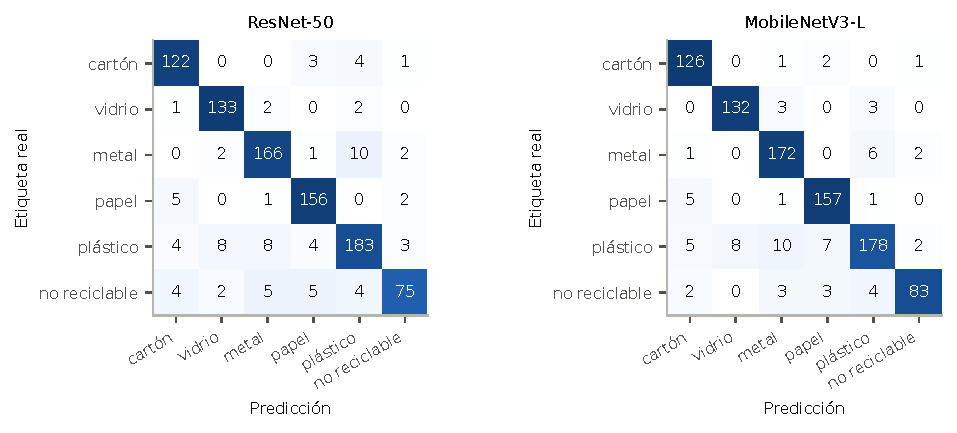
\includegraphics[width=0.66\textwidth]{confusion_matrices.pdf}
\caption{Test confusion matrices. Color indicates the proportion relative to the true class.}
\label{fig:confusion}
\end{figure*}

\begin{table*}[t]
\centering
\caption{Per-class test precision (P), recall (R), and F1 (\%)}
\label{tab:perclass}
\begin{tabular}{lrrrrrrr}
\toprule
Class & P (ResNet) & R (ResNet) & F1 (ResNet) & P (MobileNet) & R (MobileNet) & F1 (MobileNet) & $n$ \\
\midrule
cardboard & 89.7 & 93.8 & 91.7 & 90.6 & 96.9 & 93.7 & 130 \\
glass & 91.7 & 96.4 & 94.0 & 94.3 & 95.7 & 95.0 & 138 \\
metal & 91.2 & 91.7 & 91.5 & 90.5 & 95.0 & 92.7 & 181 \\
paper & 92.3 & 95.1 & 93.7 & 92.9 & 95.7 & 94.3 & 164 \\
plastic & 90.1 & 87.1 & 88.6 & 92.7 & 84.8 & 88.6 & 210 \\
non-recyclable & 90.4 & 78.9 & 84.3 & 94.3 & 87.4 & 90.7 & 95 \\
\bottomrule
\end{tabular}

\end{table*}

\subsection{Transfer Learning Strategies}

Table~\ref{tab:strategies} shows that freezing the entire extractor is the worst option for both networks. ImageNet features are not enough for materials distinguished by gloss, transparency, or texture, and fine-tuning the extractor improves macro F1 by 3.8 to 8.8 points. The three fine-tuning strategies are very close to one another. The effect of augmentation depends on the architecture: in MobileNet it improves the result, whereas in ResNet-50 partial fine-tuning without augmentation came out on top. That choice was kept because the criterion had been fixed in advance. As a consequence, the chosen ResNet is probably less tolerant of camera changes.

\begin{figure}[t]
\centering
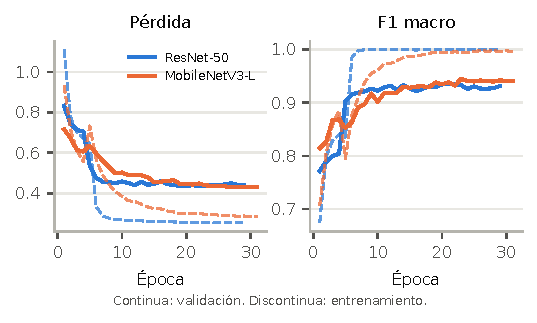
\includegraphics[width=\columnwidth]{vision_curves.pdf}
\caption{Curves of the chosen strategy for each architecture.}
\label{fig:vision-curves}
\end{figure}

In Fig.~\ref{fig:vision-curves}, the jump at epoch 5 marks the start of fine-tuning. The ResNet without augmentation reaches a training F1 of 1 within a few epochs, although its validation score remains stable. With augmentation, MobileNet's gap is smaller.

\begin{table}[t]
\centering
\caption{Classifiers on the test split}
\label{tab:vision}
\begin{tabular}{lrr}
\toprule
Métrica & ResNet-50 & MobileNetV3-L \\
\midrule
Accuracy (\%) & 91,0 & 92,4 \\
\quad IC 95\,\% & [89,0; 92,8] & [90,6; 94,0] \\
F1 macro (\%) & 90,6 & 92,5 \\
\quad IC 95\,\% & [88,5; 92,5] & [90,6; 94,1] \\
Precisión macro (\%) & 90,9 & 92,6 \\
Recall macro (\%) & 90,5 & 92,6 \\
Accuracy TrashNet (\%) & 92,9 & 93,4 \\
Accuracy RealWaste (\%) & 89,6 & 91,6 \\
Parámetros (millones) & 23,5 & 4,2 \\
Archivo, float16 (MB) & 47,2 & 8,6 \\
\bottomrule
\end{tabular}

\end{table}

\begin{figure*}[t]
\centering
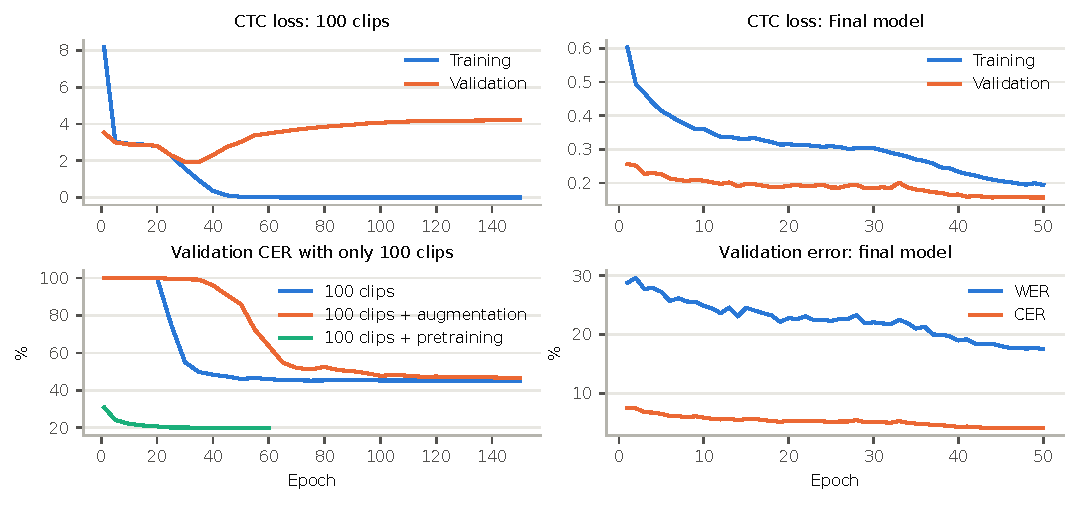
\includegraphics[width=0.74\textwidth]{speech_curves.pdf}
\caption{CTC training. Top: loss with 100 recordings and for the final model. Bottom: validation error.}
\label{fig:speech-curves}
\end{figure*}

\begin{table*}[t]
\centering
\caption{CTC experiments on the same validation set, with greedy decoding (\%). $N$: training recordings}
\label{tab:experiments}
\begin{tabular}{lrrrrr}
\toprule
Experiment & $N$ & WER unseen & CER unseen & WER TUX & CER TUX \\
\midrule
100 clips & 100 & 101.5 & 45.0 & 107.3 & 53.0 \\
100 clips + augmentation & 100 & 97.1 & 46.7 & 98.9 & 54.4 \\
TUX only (pretraining) & 10432 & 81.2 & 32.4 & 11.5 & 2.0 \\
100 clips + pretraining & 100 & 62.8 & 19.7 & 21.9 & 4.4 \\
Final model & 18779 & 29.9 & 7.8 & 10.9 & 2.0 \\
\bottomrule
\end{tabular}

\end{table*}

\subsection{Model Comparison on the Test Set}

MobileNetV3-Large achieved \MobAcc\,\% and ResNet-50 \ResAcc\,\% (Table~\ref{tab:vision}). Among the disagreements, only ResNet was correct on \McA{} images and only MobileNet on \McB{}. McNemar's test gives $p$ \McP, so \emph{neither network can be claimed to be more accurate than the other}. MobileNet was chosen for the application because of its better validation F1, its size, and its CPU latency. Both perform somewhat worse on RealWaste, where objects are dirty or deformed, but the gap with TrashNet is only a few points.

\begin{figure}[t]
\centering
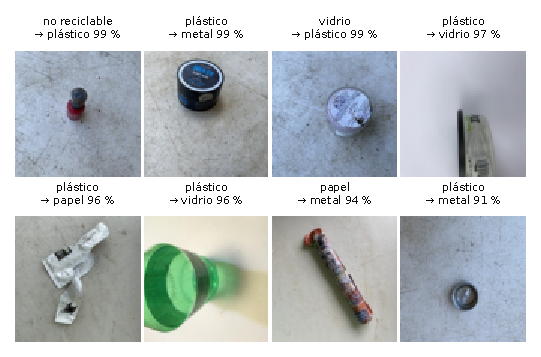
\includegraphics[width=0.78\columnwidth]{vision_errors.pdf}
\caption{Highest-confidence errors of MobileNetV3-L (true $\to$ predicted).}
\label{fig:errors}
\end{figure}

\begin{table*}[t]
\centering
\caption{Successes and failures on unseen speakers, taken from fixed positions of the WER ranking (\%)}
\label{tab:examples}
\small
\begin{tabular}{>{\raggedright\arraybackslash}p{0.44\textwidth}>{\raggedright\arraybackslash}p{0.44\textwidth}r}
\toprule
Reference & Transcription & WER \\
\midrule
ahora mismo en la isla de puerto rico hay cuarenta y cinco centros de acopio registrados & ahora mismo en la isla de puerto rico hay cuarenta y cinco centros de acopio registrados & 0 \\
me puedes mandar una foto de ella & me puedes mandar una foto de ella & 0 \\
me ayudas a plantar los naranjos & me ayudas a plantar los baranjos & 17 \\
el otro día ví un video en facebook sobre un aparatito que te ponías en la oreja y directamente te traducía & el otro día de un vida en frais por sobre en un aparatito que te ponía en la oreja y directamente de traducía & 33 \\
en el centro hay unos muy buenos bares con pantallas de plasma de sesenta pulgadas para disfrutar bien el partido & en el centro hay un es muy buenos varas con pantalla plaza de sesenta pulgas para es tu tar bien el partido & 50 \\
siempre he sido muy fan del color gris claro & siempresión muy tan el color desclaro & 78 \\
\bottomrule
\end{tabular}

\end{table*}

\subsection{Visual Error Analysis}
According to Table~\ref{tab:perclass} and Fig.~\ref{fig:confusion}, the hardest class for MobileNet is plastic, by recall: it is confused with metal (shiny surfaces), glass (transparency), paper (crumpled white packaging), and cardboard (printed containers). In ResNet, the trash (non-recyclable) class has the lowest recall. It is the smallest and most heterogeneous class, since it is defined by exclusion rather than by a material.

Fig.~\ref{fig:errors} shows the highest-confidence errors. Several are ambiguous even for a person: mixed-material containers, metal lids within the plastic class, or transparent green plastic that looks like glass. A confidence threshold does not eliminate these cases, but it does help. Calibration, with a temperature of \BestTemp{}, reduced the expected calibration error from \EceBefore\,\% to \EceAfter\,\%. With a threshold of 0.7, the model answers on \RejectCoverage\,\% of the test images and is correct on \RejectAcc\,\% of them.

\begin{table}[t]
\centering
\caption{Final model on validation and test (\%). $^{*}$\,$\alpha$ and $\beta$ were tuned on half of the validation set}
\label{tab:speech}
\resizebox{\columnwidth}{!}{\begin{tabular}{lrrrr}
\toprule
Decodificador & WER nuevos & CER nuevos & WER TUX & CER TUX \\
\midrule
Voraz & 35,1 & 9,7 & 10,8 & 1,9 \\
Beam & 35,1 & 9,6 & 10,5 & 1,8 \\
Beam + LM & 24,6 & 7,9 & 8,7 & 1,8 \\
\bottomrule
\end{tabular}
}
\end{table}

\begin{table}[t]
\centering
\caption{Test results by group, with beam search and language model (\%)}
\label{tab:speakers}
\begin{tabular}{lrrrr}
\toprule
Group & $n$ & WER & CER & Exact \\
\midrule
Unseen speakers & 278 & 24.6 & 7.9 & 17.6 \\
TUX speaker & 574 & 8.7 & 1.8 & 55.2 \\
Colombia, female & 60 & 28.0 & 9.7 & 16.7 \\
Colombia, male & 60 & 15.1 & 4.1 & 26.7 \\
Peru, female & 38 & 22.7 & 7.3 & 21.1 \\
Peru, male & 60 & 27.3 & 9.3 & 13.3 \\
Puerto Rico, female & 60 & 28.2 & 8.7 & 11.7 \\
\bottomrule
\end{tabular}

\end{table}

\subsection{Speech: What 100 Recordings Can Achieve}

From scratch, the 100 recordings lead to memorization: the training loss drops below 0.001 while the validation loss rises from its minimum (Fig.~\ref{fig:speech-curves}). The CER stalls at \ExpScratchCer\,\% and the WER at \ExpScratchWer\,\%, which exceeds 100\,\% because of insertions (Table~\ref{tab:experiments}). The curve also shows the initial phase typical of CTC: for about 20 epochs the network emits only blanks and the CER is 100\,\%.

\begin{figure}[t]
\centering
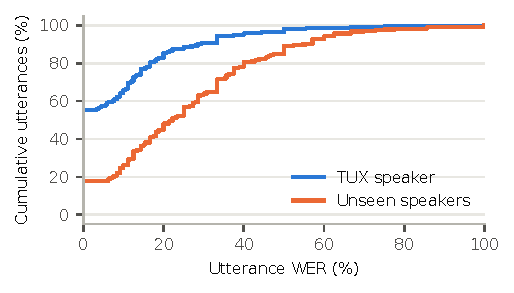
\includegraphics[width=0.70\columnwidth]{speech_distribution.pdf}
\caption{Cumulative distribution of per-utterance test WER.}
\label{fig:distribution}
\end{figure}

Data augmentation delays the exit from that phase and slows memorization, but it does \emph{not} improve the CER (\ExpAugCer\,\%). With so few examples, there is not enough variety of words and voices, and distorting the same recordings does not create it. Pretraining, in contrast, does change the outcome. The TUX model on its own fails on new voices (CER of \ExpTuxCer\,\%), but fine-tuning it on the same 100 recordings lowers the CER to \ExpTransferCer\,\%: the network already knows the mapping between Spanish sounds and letters and only needs to adapt to the voices. With the full corpus, it drops to \ExpMultiCer\,\%.

\begin{table}[t]
\centering
\caption{End-to-end latency on the demonstration machine}
\label{tab:latency}
\begin{tabular}{llr}
\toprule
Task & Hardware & Median / p95 \\
\midrule
Image, ResNet-50 & GPU & 6.1 / 8.8 ms \\
Image, MobileNetV3-L & GPU & 5.3 / 7.6 ms \\
Video 720p, ResNet-50 & GPU & 101.9 fps \\
Video 720p, MobileNetV3-L & GPU & 106.3 fps \\
5 s audio & GPU & 0.05 / 0.05 s \\
10 s audio & GPU & 0.09 / 0.10 s \\
Image, ResNet-50 & CPU & 30.2 / 32.7 ms \\
Image, MobileNetV3-L & CPU & 8.3 / 9.6 ms \\
Video 720p, ResNet-50 & CPU & 30.3 fps \\
Video 720p, MobileNetV3-L & CPU & 84.2 fps \\
5 s audio & CPU & 0.19 / 0.19 s \\
10 s audio & CPU & 0.38 / 0.39 s \\
\bottomrule
\end{tabular}

\end{table}

\subsection{Final Speech Model}

On validation, which was not used for training, the final model obtains a WER of \ValSlrWer\,\% and a CER of \ValSlrCer\,\% on unseen speakers (Table~\ref{tab:speech}). This figure is somewhat optimistic because alpha and beta were chosen on half of that set. On the test set, with unseen speakers and sentences, the WER is \SlrWer\,\% (95\,\% CI: \SlrWerLow{} to \SlrWerHigh) and the CER \SlrCer\,\%. Beam search without a language model barely changes the greedy output, because the network concentrates probability on a single path. Adding the language model lowers the WER from \SlrWerGreedy\,\% (Table~\ref{tab:speech}). The improvement is larger in WER than in CER: the n-gram corrects isolated letters and spaces that are enough to ruin a word.

With the TUX speaker, the WER is \TuxWer\,\%. The gap with respect to unseen speakers confirms that reporting only a sentence-level split would have given an overly optimistic picture. There are also marked differences between voices (Table~\ref{tab:speakers}), but each group has a single test speaker, so they reflect that person rather than a country or sex. Fig.~\ref{fig:distribution} shows the full error distribution.

In Table~\ref{tab:examples}, most failures are phonetically plausible. The most frequent character errors are missing or inserted spaces, a dropped \emph{s} (aspirated in parts of Latin American Spanish), the silent \emph{h}, confusions between \emph{b} and \emph{v}, which sound the same, and accent marks. The worst cases merge several words when speech is fast. Loanwords such as ``facebook'' fail because their spelling does not follow Spanish pronunciation.

\subsection{Video and Near Real Time}

Latency includes preprocessing, inference, and, depending on the case, video decoding, drawing, or beam search (Table~\ref{tab:latency}). All combinations exceed the thresholds of 5 frames per second and 5\,s per recording, even without a GPU. The 95th-percentile audio latency is \AudioLat\,s on GPU and \AudioLatCpu\,s on CPU. On GPU both networks are similar because preprocessing dominates. On CPU, MobileNet is more than three times faster per image. These figures do not include sending each frame to the browser.

The test video is our own montage of twelve test photos with simulated motion, rotation, and lighting changes, 62 frames per photo. MobileNet was correct on \VideoAcc\,\% of the frames. Failures concentrate on three photos that the model already misclassified as still images. Motion changed little: it corrected some frames of one of them and added some flicker, which smoothing reduces on screen. With twelve objects, this figure is a demonstration and not a performance estimate.

We also recorded two videos of our own with a phone (480$\times$864 pixels, 30 frames per second): a plastic water bottle (\OwnBottleFrames{} frames) and a notebook (\OwnNotebookFrames{} frames), on a white appliance, indoors under artificial light. Neither was used for training or tuning anything. MobileNetV3-L correctly classified \OwnBottleMob\,\% of the bottle frames and \OwnNotebookMob\,\% of the notebook frames; in the rest it confused the notebook with cardboard. ResNet-50 was correct on only \OwnBottleRes\,\% and \OwnNotebookRes\,\%: it saw glass in the transparent bottle and cardboard in the notebook. On the test set the two networks were indistinguishable, but with a real camera and outside both datasets the difference is huge. This is the clearest evidence in favor of data augmentation, which the chosen ResNet did not use, and of choosing MobileNet for the application. With two videos, it remains an observation and not a performance measurement.

\section{Conclusiones y trabajos futuros}\label{sec:conclusiones}

Sobre la primera pregunta, ajustar el extractor aporta más que cambiar de una red móvil a una grande, y el aumento de datos resultó decisivo con videos reales de celular, donde la red entrenada sin él falló casi siempre. MobileNetV3-Large alcanzó \MobAcc\,\% en prueba sin diferencia significativa con ResNet-50 (\ResAcc\,\%) y con una fracción del tamaño, por lo que la red grande no se justifica en este problema.

Sobre la segunda, 100 audios no bastan para que un DeepSpeech2 entrenado desde cero generalice, y el aumento de datos por sí solo no lo remedia. El preentrenamiento reduce el CER a menos de la mitad con los mismos 100 audios. Con un corpus de veinte horas y varios locutores se llega a un WER de \SlrWer\,\% con personas no vistas.

Sobre la tercera, un equipo de escritorio responde en tiempo casi real con las tres modalidades, y también lo hace sin GPU.

El trabajo tiene limitaciones. Las imágenes tienen fondos lisos y un objeto por foto, y el sistema no tiene una clase ``ningún objeto''. La agrupación por similitud reduce la fuga entre fotos de un mismo objeto, pero no la descarta. Solo hay un locutor de prueba por grupo. La voz es leída y no incluye acento costarricense. Solo se grabaron dos videos propios, y la aplicación no se evaluó con usuarios.

Como trabajos futuros se propone grabar, con consentimiento, un conjunto costarricense de residuos y voz, sustituir la clasificación del cuadro por detección de objetos, probar un codificador Conformer y un modelo de lenguaje de palabras, y reconocer en la voz consultas como ``dónde boto esta botella'' para unir las dos modalidades en una misma respuesta.

\section*{Use of Generative Artificial Intelligence}

This project was developed with the support of Claude (Anthropic), used as a programming agent through Claude Code. The team defined the requirements from the assignment and the course material, required that the models be trained with the methodologies seen in class and that no third-party models be presented as our own, recorded the test videos, and approved the decisions made along the way. The tool generated the experimental design, the code, the training and evaluation runs, and the analysis, and drafted this article and the presentation; the team reviewed these drafts, checked the results, and requested corrections. All figures come from real runs and can be reproduced from the repository. The team is responsible for the submitted content and for understanding and explaining every part of it.

\section*{Code, Data, and Licenses}

The code, manifests, weights, and a subset of the data are available at \url{https://github.com/KthArg/ecovoz}. The ImageNet weights and the CNN implementations come from torchvision~\cite{torchvision} (BSD-3). We also use PyTorch (BSD-3), Gradio (Apache-2.0), OpenCV (Apache-2.0), and scikit-learn (BSD-3). The speech architecture is based on the Keras example seen in class~\cite{keras-ctc} (Apache-2.0), rewritten. Derivatives of RealWaste are for non-commercial use only.

\begin{thebibliography}{00}

\bibitem{yosinski} J. Yosinski, J. Clune, Y. Bengio, and H. Lipson, ``How transferable are features in deep neural networks?'' in \emph{Advances in Neural Information Processing Systems}, vol. 27, 2014.

\bibitem{imagenet} O. Russakovsky \emph{et al.}, ``ImageNet Large Scale Visual Recognition Challenge,'' \emph{International Journal of Computer Vision}, vol. 115, pp. 211--252, 2015.

\bibitem{resnet} K. He, X. Zhang, S. Ren, and J. Sun, ``Deep residual learning for image recognition,'' in \emph{Proc. IEEE CVPR}, 2016, pp. 770--778.

\bibitem{mobilenet} A. Howard \emph{et al.}, ``Searching for MobileNetV3,'' in \emph{Proc. IEEE/CVF ICCV}, 2019, pp. 1314--1324.

\bibitem{ctc} A. Graves, S. Fernández, F. Gomez, and J. Schmidhuber, ``Connectionist temporal classification: Labelling unsegmented sequence data with recurrent neural networks,'' in \emph{Proc. ICML}, 2006, pp. 369--376.

\bibitem{beam} A. Hannun, A. Maas, D. Jurafsky, and A. Ng, ``First-pass large vocabulary continuous speech recognition using bi-directional recurrent DNNs,'' arXiv:1408.2873, 2014.

\bibitem{ds2} D. Amodei \emph{et al.}, ``Deep Speech 2: End-to-end speech recognition in English and Mandarin,'' in \emph{Proc. ICML}, 2016, pp. 173--182.

\bibitem{keras-ctc} M. R. Bouadjenek and N. D. Huynh, ``Automatic speech recognition using CTC,'' Keras Code Examples, 2021. [Online]. Available: \url{https://keras.io/examples/audio/ctc_asr/}

\bibitem{trashnet} M. Yang and G. Thung, ``Classification of trash for recyclability status,'' CS229 report, Stanford University, 2016. [Online]. Available: \url{https://github.com/garythung/trashnet}

\bibitem{realwaste} S. Single, S. Iranmanesh, and R. Raad, ``RealWaste: A novel real-life data set for landfill waste classification using deep learning,'' \emph{Information}, vol. 14, no. 12, art. 633, 2023.

\bibitem{tux} E. Jiménez Delgado, ``tux-100h,'' IC-6200 course dataset, 2022. [Online]. Available: \url{https://gitlab.com/ejimenezdelgado/tux-100h}

\bibitem{openslr} A. Guevara-Rukoz \emph{et al.}, ``Crowdsourcing Latin American Spanish for low-resource text-to-speech,'' in \emph{Proc. LREC}, 2020, pp. 6504--6513.

\bibitem{calibration} C. Guo, G. Pleiss, Y. Sun, and K. Q. Weinberger, ``On calibration of modern neural networks,'' in \emph{Proc. ICML}, 2017, pp. 1321--1330.

\bibitem{specaugment} D. S. Park \emph{et al.}, ``SpecAugment: A simple data augmentation method for automatic speech recognition,'' in \emph{Proc. Interspeech}, 2019, pp. 2613--2617.

\bibitem{gradio} A. Abid \emph{et al.}, ``Gradio: Hassle-free sharing and testing of ML models in the wild,'' arXiv:1906.02569, 2019.

\bibitem{mcnemar} Q. McNemar, ``Note on the sampling error of the difference between correlated proportions or percentages,'' \emph{Psychometrika}, vol. 12, no. 2, pp. 153--157, 1947.

\bibitem{torchvision} TorchVision maintainers and contributors, ``TorchVision: PyTorch's computer vision library,'' 2016. [Online]. Available: \url{https://github.com/pytorch/vision}

\end{thebibliography}


\end{document}
